% https://www.sharelatex.com/blog/2013/08/27/tikz-series-pt1.html

\documentclass[tikz]{standalone}
\usetikzlibrary{matrix}

\newcommand{\drawdice}[6] {%
  \matrix(m)[matrix of nodes, ampersand replacement=\&, nodes={minimum width=2em,font=\LARGE}]
  {
      \& #2 \& \& \\
      #1 \& #4 \& #5 \& #6\\
        \& #3 \& \& \\
  };
  \draw (m-3-2.south west) rectangle (m-1-2.north east);
  \draw (m-2-1.south west) rectangle (m-2-4.north east);
  \draw (m-2-3.south east) -- (m-2-3.north east);
}

\begin{document}
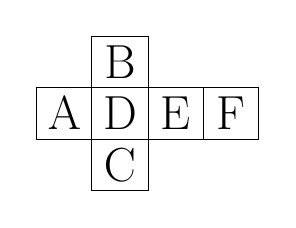
\begin{tikzpicture}[scale=2]
  \drawdice{A}{B}{C}{D}{E}{F}  
\end{tikzpicture}
\end{document}



%\begin{tikzpicture}[scale=2]
%    \tikzstyle{ann} = [draw=none,fill=none,right]
%    \matrix[nodes={draw, ultra thick, fill=blue!20},
%        row sep=0.3cm,column sep=0.5cm] {
%    \node[draw=none,fill=none] {Plain node}; &
%    \node[rectangle] {Rectangle}; &
%    \node[circle] {Circle};\\
%    \node[ellipse] {Ellipse};&
%    \node[circle split] {Circle \nodepart{lower} split};&
%    \node[forbidden sign,text width=4em, text centered]
%                    {Forbidden sign};\\
%    \node[diamond] {Diamond};&
%    \node[cross out] {Cross out};&
%    \node[strike out] {Strike out};\\
%    \node[regular polygon,regular polygon sides=5] {$n=5$};&
%    \node[regular polygon,regular polygon sides=7] {$n=7$};&
%    \node[regular polygon,regular polygon sides=9] {$n=9$};&
%    \node[ann]{Regular polygon};\\
%    \node[star,star points=4] {$p=4$};&
%    \node[star,star points=7,star point ratio=0.8] {$p=7$};&
%    \node[star,star points=10] {$p=9$};&
%    \node[ann]{Star};\\
%    };
%\end{tikzpicture}

